\chapter{Mask R-CNN}
\label{chap:maskrcnn}

In this chapter, the Mask R-CNN or Mask Region-based Convolutional Neural Network is introduced as a framework to be used to overcome the Airbus ship detection challenge.  Based on the defined classes or objects, the system detects the objects and delivers their respective masks. The image segmentation property of this framework makes it a powerful tool for the ship detection challenge. In this section, the background of the model is explored first. Afterward, the model itself together with its components will be introduced. How this model handles the data, the model and its data delivery will be inspected subsequently.  Finally, the evaluation and improvement suggestion will be provided.

\section{Related Works}
\label{sec:relatedworks}

The computer vision section has improved rapidly in object detection and semantic segmentation thanks to the baseline systems, such as Fast R-CNN \cite{Girshick15}, Faster R-CNN \cite{RenHG015} and Fully Convolutional Network (FCN) \cite{LongSD14}. Compared to the mentioned computer vision tasks, the task of image segmentation has proven to be very challenging. Due to the challenging nature of instance segmentation, the development team of the Mask R-CNN has targeted a framework for this task, which is comparable to those mentioned earlier in performance, robustness and flexibility \cite{HeGDG17}. Before diving into the framework and its components, the image segmentation and R-CNN or Region-based CNN will be explored for setting the ground of the Mask R-CNN.

\subsection{R-CNN and paving the way towards the Mask R-CNN}
\label{subsec:imagesegmentation}

The Region-based Convolutional Neural Network approach generates category-independent region proposals, called Region of Interests or RoI, by using a region proposal module. Each region is then fed individually to a CNN (part of a large CNN) which acts as a feature extraction component. The CNN extracts a fixed-length vector from each region and produces feature vectors as output, which is also fed to set of SVMs \footnote{Support Vector Machine} for classification. In other words, it trains the backbone convolutional networks separately (and end-to-end) on every single RoI to classify each RoI into object(s) of interest or background. R-CNN acts mainly as a classifier and make no prediction about object bounds \cite{GirshickDDM13}.

\begin{figure}[h!]
  \centering
  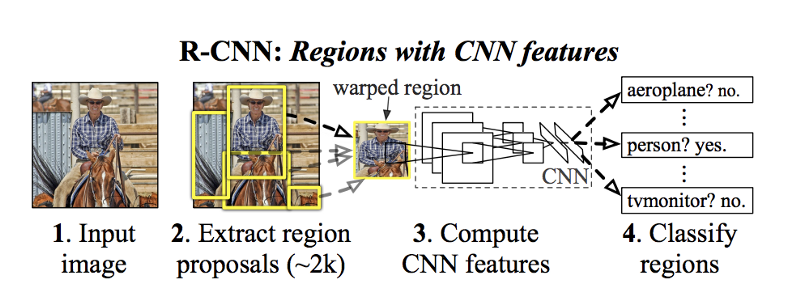
\includegraphics[width=\textwidth]{rcnn}
  \caption[R-CNN]
   {R-CNN Framwork \cite{GirshickDDM13}}
   \label{fig:rcnn}
\end{figure}
\noindent
This method was further improved to enable the attending of RoIs on feature maps by utilizing the RoI Pool, which led to a better performance and accuracy, hence the name Fast R-CNN. In Fast R-CNN, the input of the system is an entire image and a set of object proposals or RoIs. This input is processed by a large CNN together with a max pooling layer. This process pools each RoI into a fixed-sized (convolutional) feature map (containing only RoIs). By using a RoI pooling layer and a sequence of fully connected layers, each RoI on the feature map is then mapped onto a fixed-length feature vector. Finally, a softmax layer predict the class of proposed region and the offset values for the bounding box \cite{Girshick15}.

\begin{figure}[h!]
  \centering
  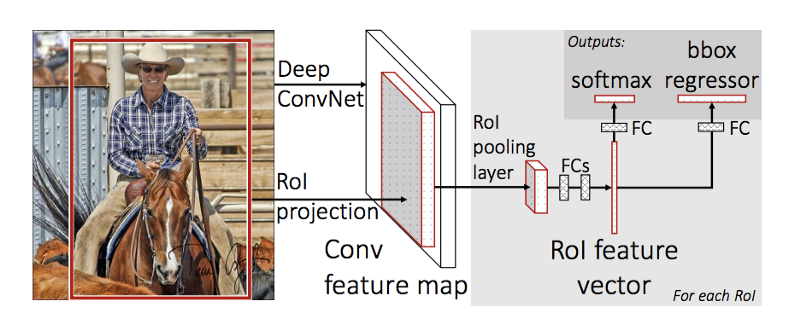
\includegraphics[width=\textwidth, height=5cm]{fast_rcnn}
  \caption[Fast R-CNN]
   {Fast R-CNN Framwork \cite{Girshick15}}
   \label{fig:fast-rcnn}
\end{figure}

\newpage
\noindent
The both mentioned methods uses selective search to generate region proposals, which is a time-consuming task. The Faster R-CNN speeds up the whole process by omitting the selective search algorithm and letting the network learn the region proposal itself. In Faster R-CNN, the system is comprised of a deep fully convolutional network which serves as region proposal module and a Fast R-CNN detector. In this case, the RPN \footnote{Region-based Proposal Network} module  ( utilizing the attention mechanism \cite{ChorowskiBSCB15})  point the regions out to Fast R-CNN module. The RPN module uses sliding-window method and scans over the convolutional feature map, which is generated by the last shared convolutional layer. Multiple region proposals are predicted at the location of each sliding-window which are called anchors. Each anchor (region proposal) is provided with a score that estimates the probability of object or not object \cite{RenHG015}.

\begin{figure}[h!]
  \centering
  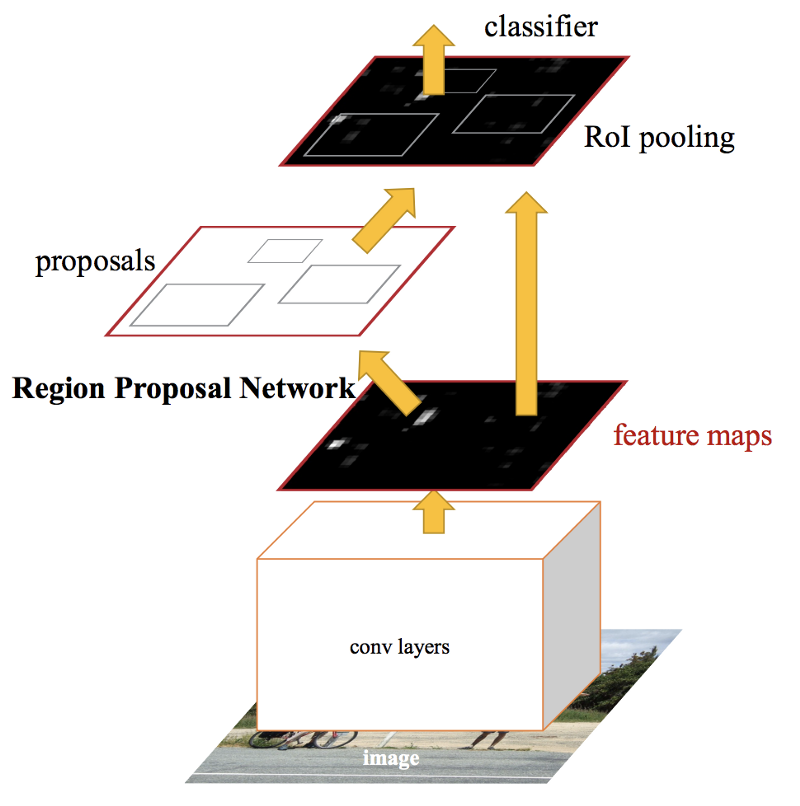
\includegraphics[scale=0.30]{faster_rcnn}
  \caption[Faster R-CNN]
   {Faster R-CNN Framwork \cite{RenHG015}}
   \label{fig:faster-rcnn}
\end{figure}


\subsection{Image Segmentation}
\label{subsec:imagesegmentation}
\noindent
Image segmentation is the process of dividing a digital image into multiple regions or segments, which correspond to different objects or parts of objects. Every pixel in the image is assigned a label which correspond to an object or a class. As a result, a set of pixels, which are labeled identically, shares a specific character. This provides a mean to represent a digital image into a much more meaningful and easier to analyze object \cite{kale2010computer}. 

\begin{figure}[t]
  \centering
  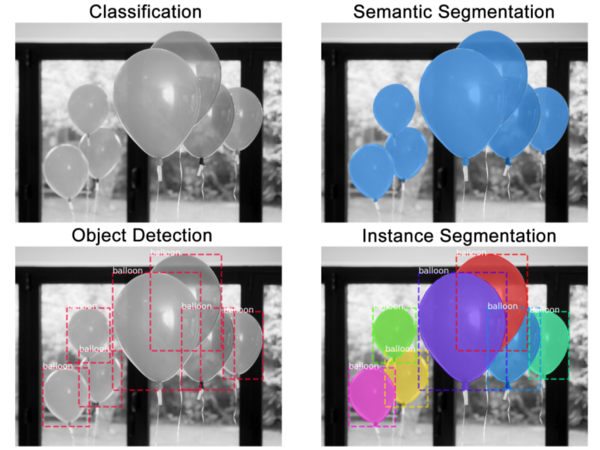
\includegraphics[scale=0.50]{image_segmentation}
  \caption[Image Segmentation]
   {Tasks of Computer Vision  \cite{imgseg}}
   \label{fig:faster-rcnn}
\end{figure}


\section{Mask R-CNN Details}
\label{sec:maskrcnn-details}

The Mask Region-based Convolutional Neural Network adopts the two-stages procedure of Fast R-CNN. It keeps the RPN stage untouched but adds a branch in parallel to the class and boundary box prediction in second stage, which outputs a binary mask for each RoI\cite{HeGDG17}. The Mask R-CNN framework, which is used for ship detection during this project, was introduced by Kaiming et al., 2017 in Mask R-CNN paper.

\begin{figure}[h!]
  \centering
  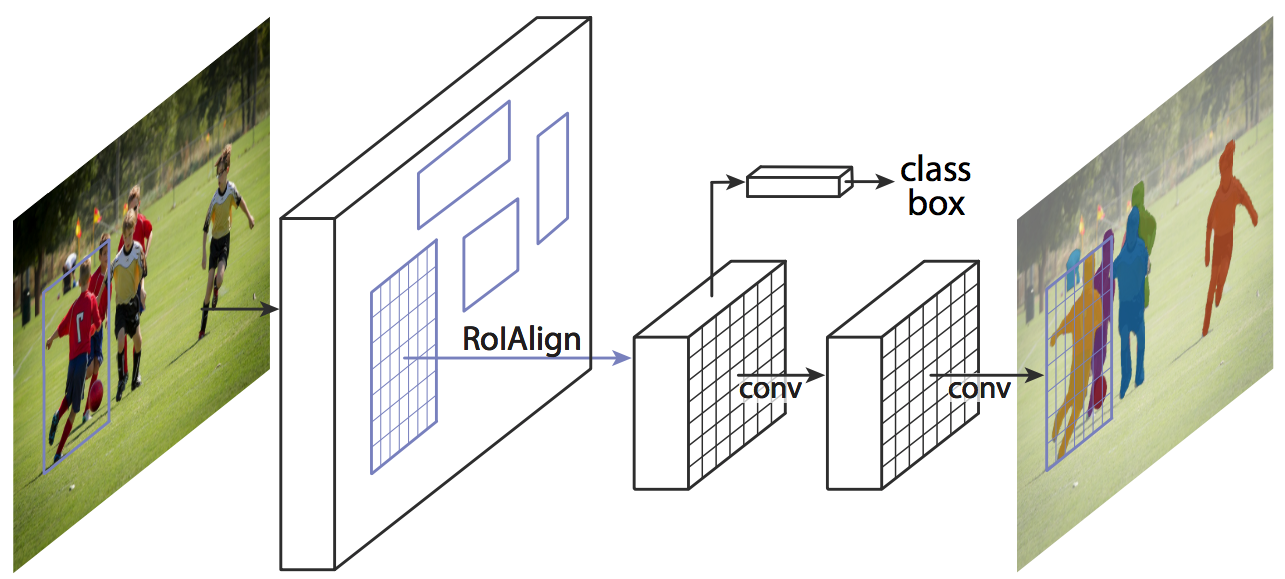
\includegraphics[scale=0.30]{maskrcnn_framework}
  \caption[Mask R-CNN]
   {Mask R-CNN Framwork \cite{HeGDG17}}
   \label{fig:faster-rcnn}
\end{figure}
\noindent
The implementation of the model is provided by Waleed A. via his Github page \cite{matterport_maskrcnn_2017}. The model is generated by using the\textbf{\textit{ Model Class API}} of \textbf{\textit{Keras}}. This framework consists of the following components:
\newpage
\begin{enumerate}
  \item \textbf{Backbone} which is composed of a standard ResNet50 or Resnet101\footnote{Residual Network which employes deep residual learning to overcome the saturation of accuracy in much deeper networks when depth of  network increases\cite{DBLP}} and is configurable in code. This component serves as a feature extractor and is extended via Feature Pyramid Network(FPN). The backbone is implemented in \textbf{\textit{Keras}}. The ResNet has 5 stages. The first stage is a keras 2D convolution layer with output filters of 64, kernel size of (7,7), ReLU function as activation and max-pooling with a pool size of (3, 3). The second stage consists of a convolution block\footnote{A residual block with shortcut which has a convolutional layer at the shortcut since input and output have different dimensions} and two identity blocks\footnote{A residual block whose shortcut can be directly used because input and output are of the same dimension} each with kernel size 3. The third stage has one convolution block and three identity blocks each also with kernel size 3. The fourth stage makes the difference between ResNet50 and 101. In our case, namely ResNet50, this stage consists of a a convolution block and five identity blocks. The last stage is  like the second stage but with diffrent output filters for convolution and identity blocks.
  \item \textbf{Region Proposal Network} or \textbf{RPN} which slides a small neural network over the generated convolutional feature map and produces anchors at each sliding-window. This layer consists of 2D CNNs and uses \textbf{\textit{soft max}} for activation.  
  \item \textbf{RoI Classifier} and \textbf{Bounding Box Regression} which runs over the RoIs generated by RPN and outputs two properties for each RoI, Class and Bounding Box Refinement. This layer is a fully connected layer(FC) and uses ReLU function for activation. 
  \item \textbf{RoI Pooling} which cropps and resizes the corresponding part of the convolutional feature map to a fixed size for feedind into the classifie.
  \item \textbf{Segmentation Masks} which is a convolutional network and generates the binary mask for each (positive) RoI selected by RoI classifier             
\end{enumerate}

\noindent
Before diving deeper in this project, it should be mentioned that the code to this project is accessible under our GitHub Repository under the URL: \url{https://github.com/mozzhorin/ML-PR18}

\section{Data}
\label{sec:data}

the train data set consists of 104070 Satellite images with the resolution of 768 x 768 pixels\footnote{the data set used for training was provided prior to changes due to the data leak\cite{dataleak}}. The training images include either ships or no ships which is indicated by masks via Run-Length-Coding . A CSV file was provided by Kaggle which contains the corresponding masks for each image. An Example of this file is shown in figure~\ref{fig:rlemask}. This data set was divide into 90\% or 93663 images for training and 10\% (10407 images) for evaluation during the training phase. Hence the number of steps per epochs and evaluation. The test data set has 15606 images with the same resolution as training data.
\begin{figure}[h!]
  \centering
  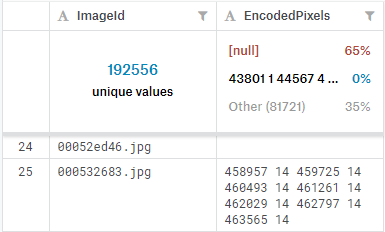
\includegraphics[scale=0.9]{train_csv_sample}
  \caption[Example of Run-Length-Coding mask]
   {Example of Run-Length-Coding mask}
   \label{fig:rlemask}
\end{figure}

\section{Hardware Configuration}
\label{sec:hardwareconfig}

For the Maks R-CNN section of the project, a system with following configuration was employed:
\begin{itemize}
\item CPU: 12 Cores (24 Threads), each core running at max clock of 4 Ghz (AMD Threadripper 1920x)
\item RAM: 32 GB DDR4 @ 3200 MHz
\item GPU: Nvidia GTX 1080ti with 11 GB of GDDR5X video memory (Pascal with 3584 CUDA cores and boost clock of 1950 MHz)
\item OS: Ubuntu 18.04
\item Development Environment: Inside a Docker container generated via official TensorFlow docker image
\end{itemize}

\section{Framework Configuration}
\label{sec:framworkconfig}

As backbone, a RestNet50 was employed in Model. As a side note, it should be mentioned that we have implemented a ResNet20, a residual Network with 20-layer residual, for gaining a better performance in training. In comparison to ResNet50, we have improved the training performance per epoch on the configuration which was mentioned in previous section(~\ref{sec:hardwareconfig}), but not significantly. Prior to these changes, the model with all its layer was already trained for 6 epochs with relative good results. Due to the insignificant improvement in performance and advancement in training, we decided to continue with the RestNet50. Arguably, a residual network is more suitable for detection of more complex objects and more number of classes. For this project, a much simpler neural network could be also utilized with even better performance. But this was also a motivation to observe if sacrificing some performance is an acceptable trade-off for gaining more accurate detection. Further configurations of the framework are as follow:
\begin{itemize}
\item Backbone: ResNet50
\item Batch size: 1 (1 image per GPU because of the resolution of the images)
\item Number of epochs: 30 (Early stoping after 6 epochs)
\item Number of steps per epoch: 93663 (due to the batch size and 90\% of training data set for training)
\item Number of validation steps:  10407 (due to the batch size and 10\% of training data set for evaluation)
\item Number of RoIs per image: 200
\item Positive RoI ratio: 0.33
\item Learning rate: 0.001
\item Learning momentum:  0.9
\item Weight decay: 0.0001
\item Detection minimum confidence: 0.90
\item Mask resized: from 768x768 to 384x384
\item Image augmentation: not employed
\end{itemize}

\section{Data Preparation}
\label{sec:datapreparation}

Initially, the images are loaded together with their corresponding masks.
\begin{figure}[h!]
  \centering
  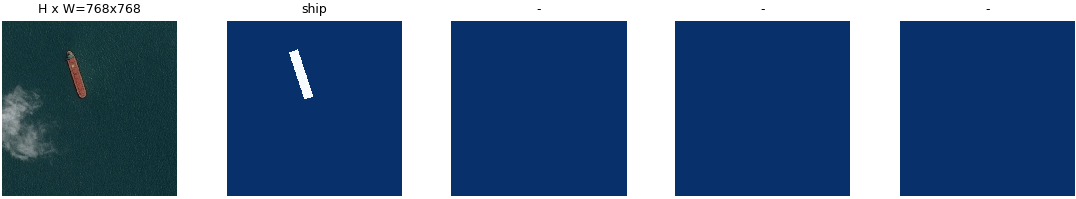
\includegraphics[width=\linewidth]{image_withMasks_0}
  \caption[Random image with mask]
   {Image with mask}
   \label{fig:rndimg}
\end{figure}
\newpage
\noindent
The bounding boxes are then computed from provided masks. To improve the training performance, the mask pixels inside the computed bounding box is stored rather than the mask of entire image. This mask is further resized to smaller size, in our case half of the original resolution. Choosing smaller masks leads to losing smaller objects. This is governed by \textbf{\textit{mini\_mask}} in config class. 

\begin{figure}[!htb]
\minipage{0.6\textwidth}
  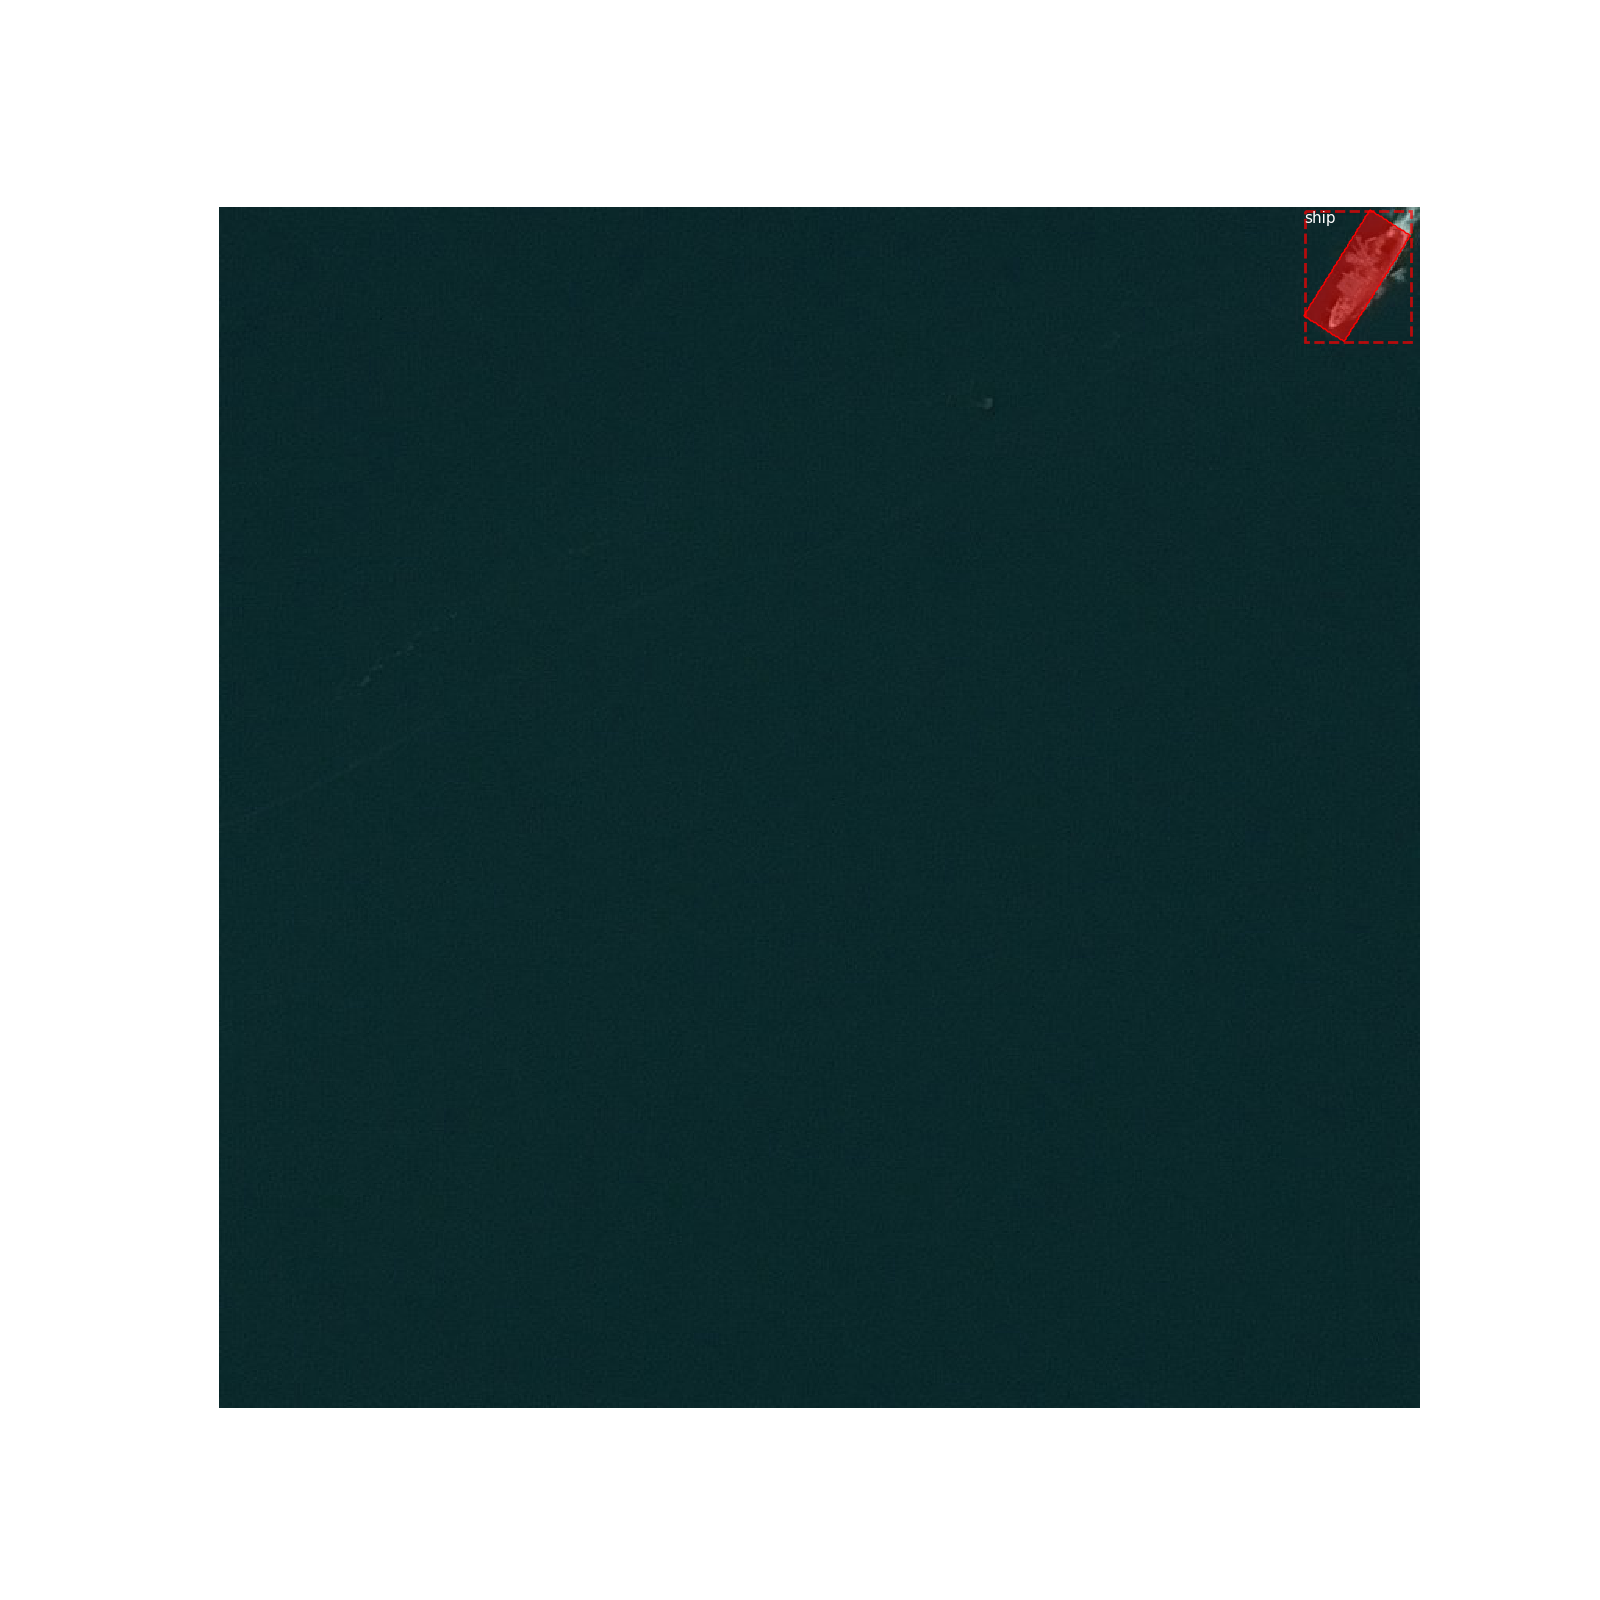
\includegraphics[width=\linewidth]{img_0_with_bounding_box}
  \caption[Iimage with bounding box]{Iimage with bounding box}\label{fig:imgbbx}
\endminipage\hfill
\minipage{0.3\textwidth}
  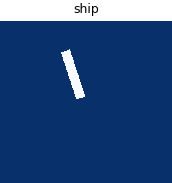
\includegraphics[scale=.7]{image_bbxwithMasks}
  \caption[The espective Mask]{The respective Mask}\label{fig:maskofbbx}
\endminipage\hfill
\end{figure}

\noindent
During the training, the method \textbf{\textit{data\_generator}} of the class model generates the following data for each instance of an object, in our case ship, on the image:

\begin{itemize}
\item The RPN generates the anchors using the sliding-window method. Initialized by method \textbf{\textit{build\_rpn\_model}}, governed by \textbf{\textit{RPN\_ANCHOR\_SCALES}} and \\ \textbf{\textit{RPN\_ANCHOR\_RATIOS}} of config class. The RoIs are generated(Fig.~\ref{fig:randomrois}) and consequently the positive anchors and their refinement(Fig. ~\ref{fig:posanchors}). 
\item Based on the positive RoIs, the classifier calculates the bounding box of an object (dotted box) and applies refinement (box with solid lines) to it(Fig.~\ref{fig:imgbbx}). The classifier is initiated via the method \textbf{\textit{fpn\_classifier\_graph()}}
\item The mask branch takes the positive regions selected by the RoI classifier and generates masks respectively(Fig.~\ref{fig:maskofbbx}). This branch is a convolutional network and is initialized by the method \textbf{\textit{build\_fpn\_mask\_graph()}}
\end{itemize}
\begin{figure}[!htb]
\minipage{0.30\textwidth}
  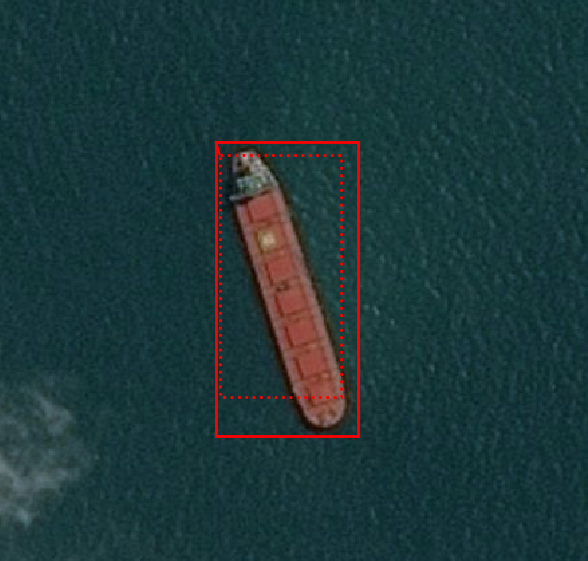
\includegraphics[width=\linewidth]{pos_ancher_img}
  \caption[Image with positive anchors]{Image with positive anchors}\label{fig:posanchors}
\endminipage\hfill
\minipage{0.30\textwidth}
  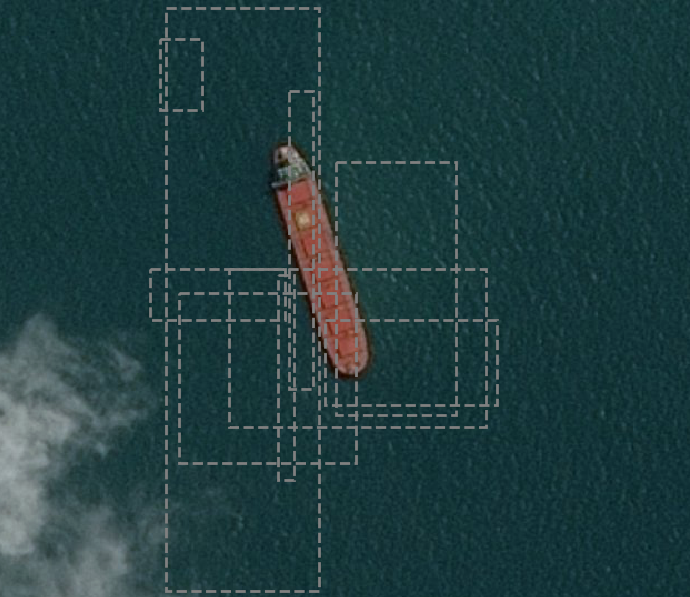
\includegraphics[width=\linewidth]{all_random_rois_img}
  \caption[Image with random RoIs]{Image with RoIs(showing 10 random RoIs out of 200)}\label{fig:randomrois}
\endminipage\hfill
\minipage{0.30\textwidth}
  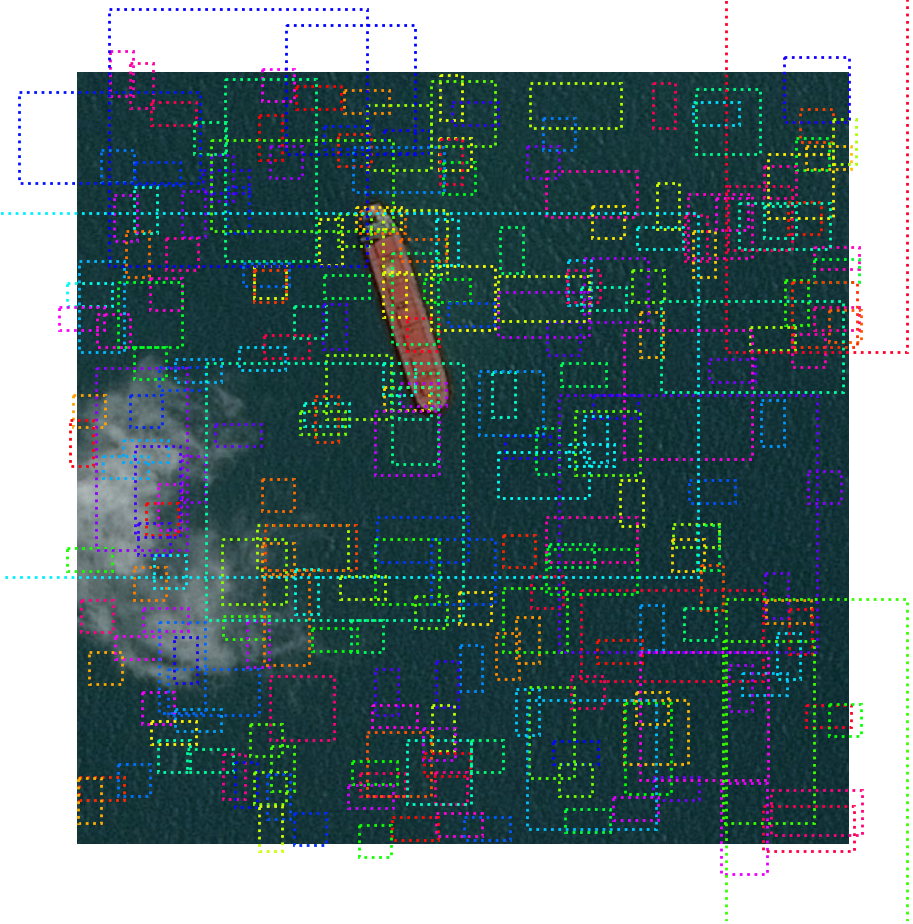
\includegraphics[width=\linewidth]{image_negative_anchors_1}
  \caption[Image with negative anchors]{Image with negative anchors}\label{fig:neganchors}
\endminipage
\end{figure}
\newpage
\section{Training}
\label{sec:training}
With the described configuration in earlier sections, each epoch took about 9 hours to complete. Due to the time constraint and relative good results, the training was stoped early after 6 epochs. 

\section{Detection}
\label{sec:detection}

The detection method of the class model predicts/detects the ships and outputs the masks and bounding boxes respectively. Some examples of generated masks are shown in the following images:
\begin{figure}[!htb]
\centering
\begin{minipage}{.5\textwidth}
  \centering
  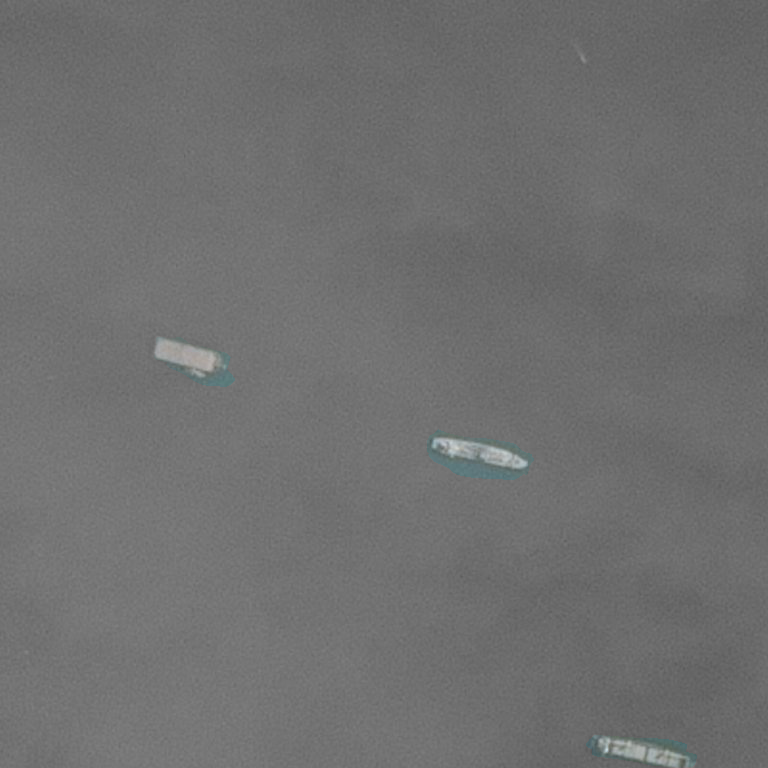
\includegraphics[width=.4\linewidth]{0a40de97d_detected_20181006T053628}
  \captionof{figure}{Grey Image}
  \label{fig:test1}
\end{minipage}%
\begin{minipage}{.5\textwidth}
  \centering
  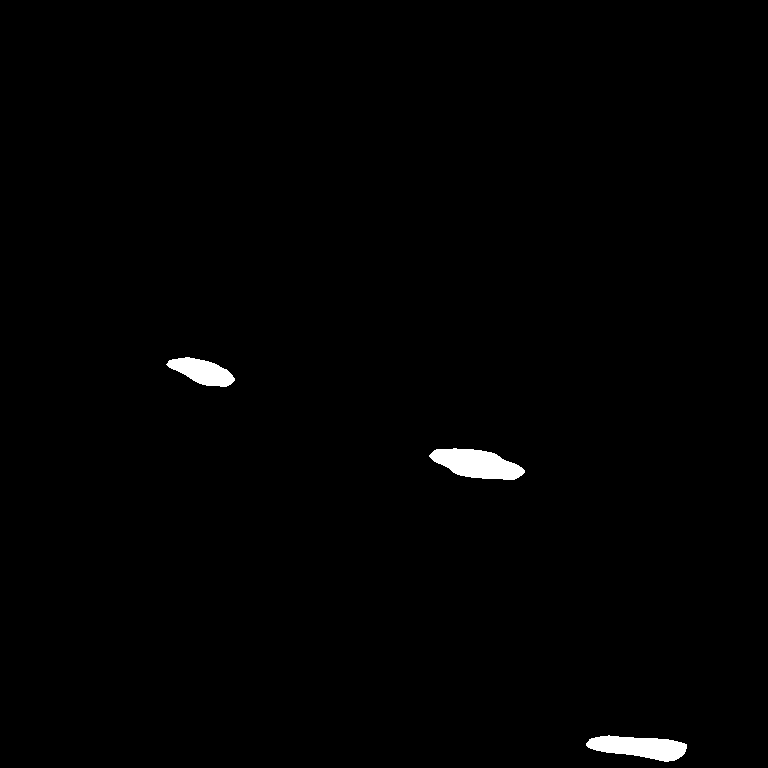
\includegraphics[width=.4\linewidth]{0a40de97d_mask_0_20181006T053628}
  \captionof{figure}{Mask of image}
  \label{fig:test2}
\end{minipage}
\end{figure}

\begin{figure}[!htb]
\centering
\begin{minipage}{.5\textwidth}
  \centering
  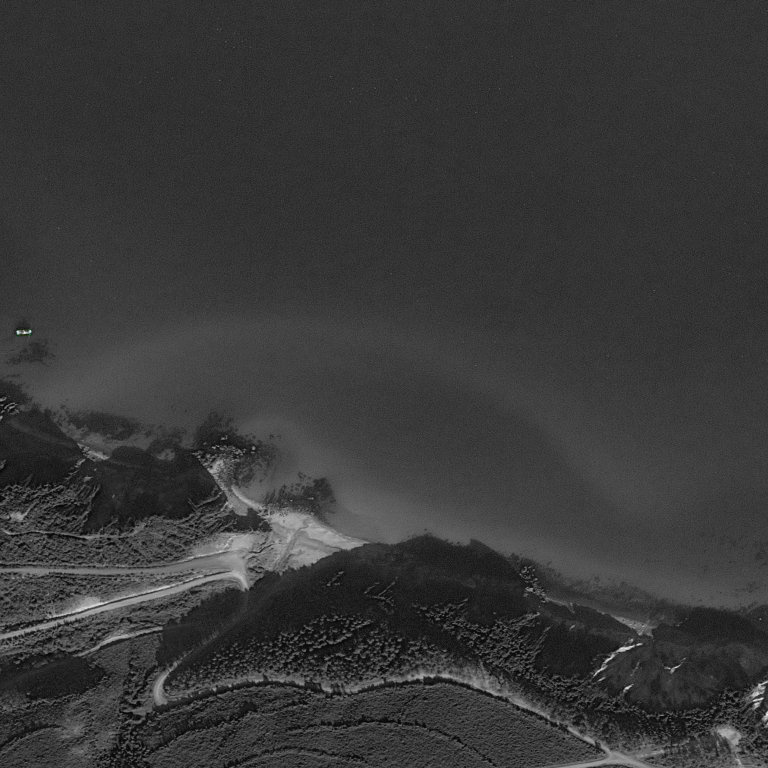
\includegraphics[width=.4\linewidth]{0abd1903b_detected_20181006T053635}
  \captionof{figure}{Image with small ship}
  \label{fig:test1}
\end{minipage}%
\begin{minipage}{.5\textwidth}
  \centering
  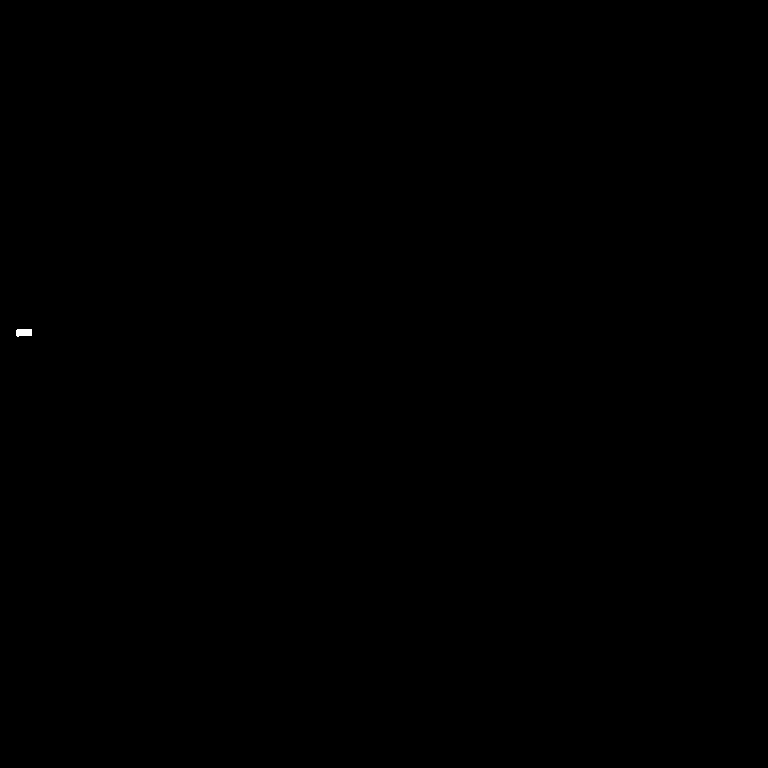
\includegraphics[width=.4\linewidth]{0abd1903b_mask_0_20181006T053635}
  \captionof{figure}{Mask of smaller ships}
  \label{fig:test2}
\end{minipage}
\end{figure}

\section{Evaluation}
\label{sec:evaluation}

\subsection{Loss}
\label{subsec:loss}

The losses of various layers of the model were recorded during training and validation and are shown in the following graphs.

\begin{figure}[!htb]
\centering
\begin{minipage}{.5\textwidth}
  \centering
  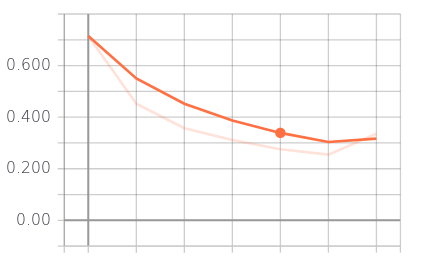
\includegraphics[width=.8\linewidth]{train_loss}
  \captionof{figure}{Train loss(Cross-Entropy)}
  \label{fig:trainloss}
\end{minipage}%
\begin{minipage}{.5\textwidth}
  \centering
  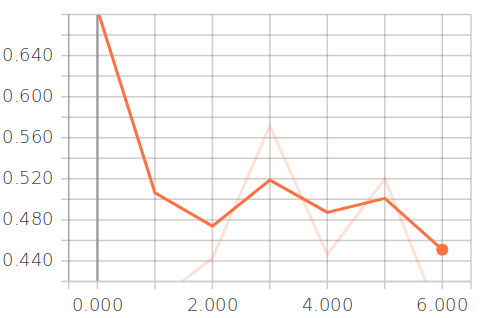
\includegraphics[width=.8\linewidth]{loss_evaluation}
  \captionof{figure}{Evalutaion loss}
  \label{fig:evaluationloss}
\end{minipage}
\end{figure}

\begin{figure}[!htb]
\centering
\begin{minipage}{.5\textwidth}
  \centering
  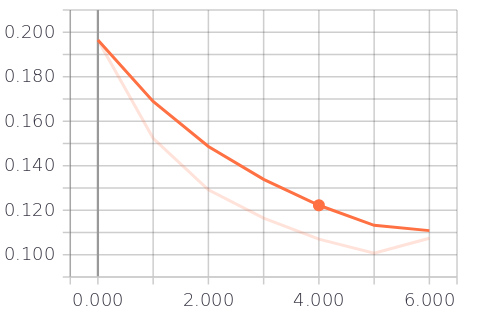
\includegraphics[width=.8\linewidth]{mask_loss_training}
  \captionof{figure}{Mask loss (Cross-Entropy) training}
  \label{fig:masktrainloss}
\end{minipage}%
\begin{minipage}{.5\textwidth}
  \centering
  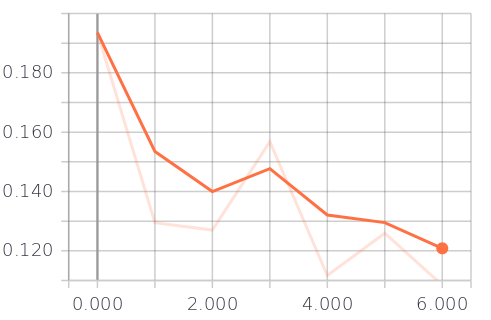
\includegraphics[width=.8\linewidth]{mask_loss_evaluation}
  \captionof{figure}{Mask loss evaluation}
  \label{fig:maskevaluationloss}
\end{minipage}
\end{figure}

\begin{figure}[!htb]
\centering
\begin{minipage}{.5\textwidth}
  \centering
  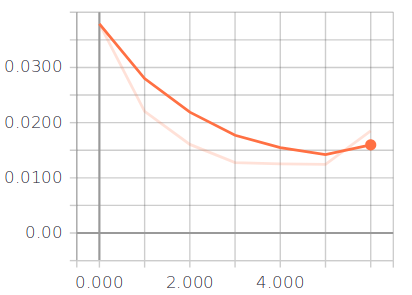
\includegraphics[width=.9\linewidth]{class_loss_training}
  \captionof{figure}{Class loss (Cross-Entropy) training}
  \label{fig:classtrainloss}
\end{minipage}%
\begin{minipage}{.5\textwidth}
  \centering
  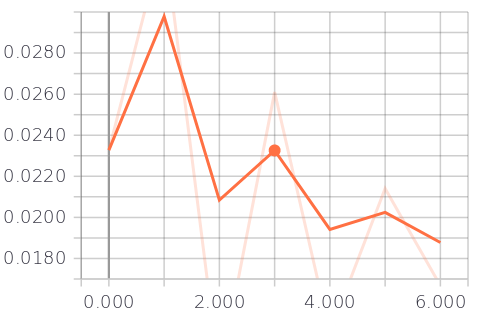
\includegraphics[width=.9\linewidth]{calss_loss_evaluation}
  \captionof{figure}{Class loss evaluation}
  \label{fig:classevaluationloss}
\end{minipage}
\end{figure}

\begin{figure}[!htb]
\centering
\begin{minipage}{.5\textwidth}
  \centering
  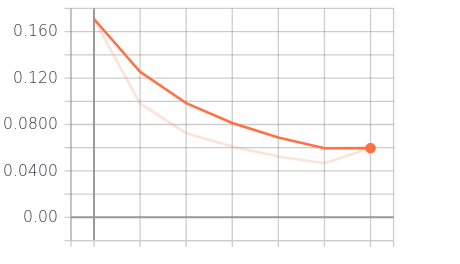
\includegraphics[width=\linewidth]{bbox_train_loss}
  \captionof{figure}{Bounding box loss training}
  \label{fig:bboxtrainloss}
\end{minipage}%
\begin{minipage}{.5\textwidth}
  \centering
  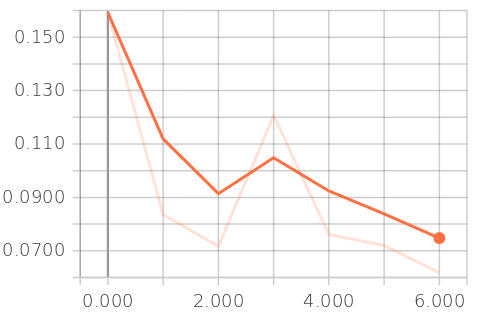
\includegraphics[width=.8\linewidth]{bbox_loss_evaluation}
  \captionof{figure}{Bounding box loss evaluation}
  \label{fig:bboxevaluationloss}
\end{minipage}
\end{figure}


\newpage
\subsection{Kaggle Score}
\label{subsec:score}

The predicted masks were encoded to Run-Length values and those values were saved in a csv file in the form of ~\ref{fig:rlemask}. 
The predictions were generated for 3 sets of test data and uploaded. The data sets and their respective results are as follow:  
\begin{enumerate}
  \item The entire test data, namly 15606 test images. The prediction/detection took about 1822 Seconds. The prediction generated the score 0.671 and positioned us at number 117
  \item the pre-classified test data with threshold 0.4 consisting of 10164 images. The prediction process took 1217 Seconds and scored 0.674 which improved our ranking to 116
  \item the pre-classified test data with threshold 0.5 consisting of 5414 images. The prediction process took 648 Seconds and generated the same score 0.674
\end{enumerate}

\begin{figure}[h!]
  \centering
  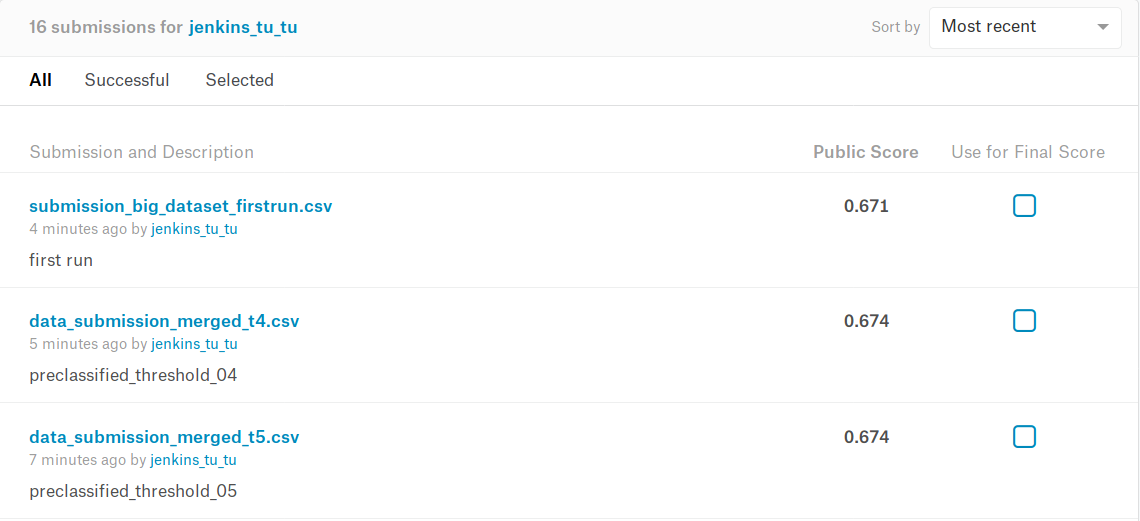
\includegraphics[width=\textwidth]{submission_score}
  \caption[Submission Scores]
   {Submission Scores}
   \label{fig:scores}
\end{figure}

\begin{figure}[h!]
  \centering
  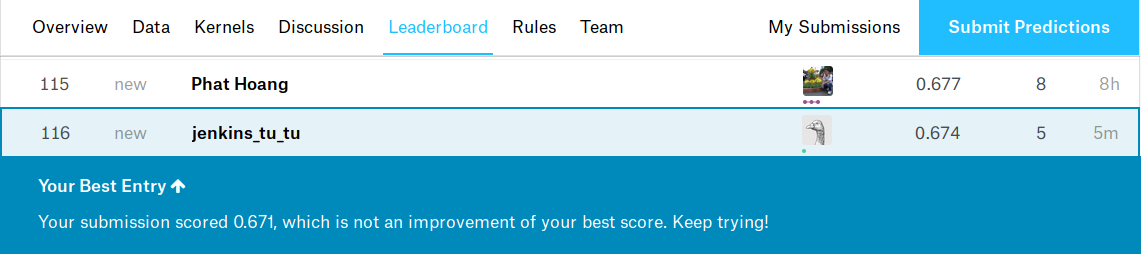
\includegraphics[width=\textwidth]{kaggle_rank}
  \caption[Kaggle Ranking]
   {Kaggle Ranking}
   \label{fig:rank}
\end{figure}


\subsection{Summary}
\label{subsec:sum}

Based on the evaluation and loss values, it is obvious that this model can provide good results if it's trained adequately.After the 6th epoch, the values of evaluation losses have declined to a good extent, which indicates an improvment in learning the data.
































